
\de{ĐỀ THI HỌC KỲ I NĂM HỌC 2022-2023}{THPT Tân Bình}

\begin{center}
	\textbf{PHẦN 1 - TRẮC NGHIỆM}
\end{center}



\Opensolutionfile{ans}[ans/ans]
%Câu 1...........................
\begin{ex}%[0T1B1-5]%[Dự án đề kiểm tra HKI1 NH22-23- Nguyễn Ngọc Nguyên]%[THPT Tân Bình]
	Cho mệnh đề \lq\lq $\forall x \in \mathbb{R} \colon x^2+x>0$\rq \rq. Mệnh đề phủ định của mệnh đề này là
	\choice
	{$\exists x \in \mathbb{R} \colon x^2+x<0$}
	{\True $\exists x \in \mathbb{R} \colon x^2+x\le 0$}
	{$\exists x \in \mathbb{R} \colon x^2+x = 0$}
	{$\forall x \in \mathbb{R} \colon x^2+x \le 0$}
	\loigiai{
Ta có mệnh đề phủ định là \lq \lq $\exists x \in \mathbb{R} \colon x^2+x\le 0$\rq \rq.		
	}
\end{ex}

\begin{ex}%[0T3B1-1]%[Dự án đề kiểm tra HKI1 NH22-23- Nguyễn Ngọc Nguyên]%[THPT Tân Bình]
	Cho hàm số $f(x)= \heva{&\dfrac{2\sqrt{x-2}-3}{x-1}  &\text{khi} \ &x \ge 2 \\ &x^2+2 & \text{khi}  \ & x <2}$. Tính $P=f(2)+f(-2)$.
	\choice
	{\True $P=3$}
	{$P=2$}
	{$P=\dfrac{7}{2}$}
	{$P=6$}
	\loigiai{
	Ta có $P=f(2)+f(-2)=\dfrac{2\sqrt{2-2}-3}{2-1}+(-2)^2+2=3$.	
	}
\end{ex}
\begin{ex}%[0T3B1-4]%[Dự án đề kiểm tra HKI1 NH22-23- Nguyễn Ngọc Nguyên]%[THPT Tân Bình]
\immini{Cho hàm số bậc hai có bảng biến thiên như hình vẽ. Hàm số này nghịch biến trên	
}
{

\begin{tikzpicture}[scale=1, font=\footnotesize,line join=round, line cap=round,>=stealth]
	\tkzTabInit[nocadre=false,lgt=1.2,espcl=2.5,deltacl=0.6]{$x$/0.8,$y$/1.8}
	{$-\infty$,$1$,$+\infty$}
	\tkzTabVar{-/$-\infty$,+/$21$,-/$-\infty$}
\end{tikzpicture}	\\
}
	\choice
	{\True $(1;+\infty)$}
	{$(-\infty;21)$}
	{$(-\infty;1)$}
	{$(-21;+\infty)$}
	\loigiai{
Từ bảng biến thiên ta thấy mũi tên đi xuống trên khoảng $(1;+\infty)$ nên hàm số nghịch biến trên $(1;+\infty)$. 		
	}
\end{ex}


\begin{ex}%[0T5Y4-1]%[Dự án đề kiểm tra HKI1 NH22-23- Nguyễn Ngọc Nguyên]%[THPT Tân Bình]
	Cho hai véc-tơ $\overrightarrow{a}$ và $\overrightarrow{b}$ tùy ý khác $\overrightarrow{0}$. Khẳng định nào dưới đây là đúng?
	\choice
	{$\overrightarrow{a} \cdot \overrightarrow{b}=\left| \overrightarrow{a} \right | \cdot \left| \overrightarrow{b} \right |$}
	{$\overrightarrow{a} \cdot \overrightarrow{b}=- \left| \overrightarrow{a} \right |\cdot \left | \overrightarrow{b} \right |$}
	{$\overrightarrow{a} \cdot \overrightarrow{b}=\left| \overrightarrow{a} \right | \cdot \left| \overrightarrow{b} \right | \cdot \sin \left(\overrightarrow{a}, \overrightarrow{b} \right)$}
	{\True $\overrightarrow{a} \cdot \overrightarrow{b}=\left| \overrightarrow{a} \right | \cdot \left| \overrightarrow{b} \right | \cdot \cos \left(\overrightarrow{a}, \overrightarrow{b} \right)$}
	\loigiai{
Theo lý thuyết ta có  $\overrightarrow{a} \cdot \overrightarrow{b}=\left| \overrightarrow{a} \right | \cdot \left| \overrightarrow{b} \right | \cdot \cos \left(\overrightarrow{a}, \overrightarrow{b} \right)$.		
	}
\end{ex}
\begin{ex}%[0T5Y2-1]%[Dự án đề kiểm tra HKI1 NH22-23- Nguyễn Ngọc Nguyên]%[THPT Tân Bình]
	Cho ba điểm $A$, $B$, $C$ phân biệt tùy ý. Khẳng định nào sau đây là đúng?
	\choice
	{$\overrightarrow{AB}-\overrightarrow{AC}=\overrightarrow{BC}$}
	{$\overrightarrow{AB} +\overrightarrow{BC}=\overrightarrow{CA}$}
	{\True $\overrightarrow{AB}-\overrightarrow{AC}=\overrightarrow{CB}$}
	{$\overrightarrow{AB} + \overrightarrow{AC}=\overrightarrow{BC}$}
	\loigiai{
Theo quy tắc ba điểm đối với phép hiệu hai véc-tơ ta có $\overrightarrow{AB}-\overrightarrow{AC}=\overrightarrow{CB}$.		
	}
\end{ex}

\begin{ex}%[0T5B1-3]%[Dự án đề kiểm tra HKI1 NH22-23- Nguyễn Ngọc Nguyên]%[THPT Tân Bình]
	Cho hai véc-tơ $\overrightarrow{a}$, $\overrightarrow{b}$ tùy ý khác $\overrightarrow{0}$. Hai véc-tơ $\overrightarrow{a}$, $\overrightarrow{b}$ được gọi là đối nhau nếu
	\choice
	{chúng ngược hướng}
	{chúng cùng phương, cùng độ dài}
	{chúng cùng hướng và cùng độ dài}
	{\True chúng ngược hướng và cùng độ dài}
	\loigiai{
Theo định nghĩa hai véc-tơ đối nhau ta có: Hai véc-tơ $\overrightarrow{a}$, $\overrightarrow{b}$ được gọi là đối nhau nếu chúng ngược hướng và cùng độ dài. 		
	}
\end{ex}
\begin{ex}%[0T4B2-1]%[Dự án đề kiểm tra HKI1 NH22-23- Nguyễn Ngọc Nguyên]%[THPT Tân Bình]
	Cho tam giác $ABC$. Chọn khẳng định đúng.
	\choice
	{$AB^2=AC^2+BC^2+2AC\cdot BC \cdot \tan A$}
	{\True $AB^2=AC^2+BC^2-2AC\cdot BC \cdot \cos C$}
	{$AB^2=AC^2+BC^2+2AC\cdot BC \cdot \cos C$}
	{$AB^2=AC^2+BC^2-2AC\cdot BC \cdot \cot A$}
	\loigiai{
Theo định lý cô-sin trong tam giác $ABC$ ta có  $AB^2=AC^2+BC^2-2AC\cdot BC \cdot \cos C$.		
	}
\end{ex}

\begin{ex}%[0T2B1-2]%[Dự án đề kiểm tra HKI1 NH22-23- Nguyễn Ngọc Nguyên]%[THPT Tân Bình]
Cặp số $(x;y)$ nào sau đây là một nghiệm của bất phương trình $2022x-2023y>0$?
	\choice
	{$(1;1)$}
	{$(-1;0)$}
	{\True $(1;0)$}
	{$(0;1)$}
	\loigiai{
Thay $x=1$ và $y=0$ vào bất phương trình ta được $2022>0$ (đúng). Do đó $(1;0)$ là một nghiệm của phương trình. 		
	}
\end{ex}

\begin{ex}%[0T1B3-1]%[Dự án đề kiểm tra HKI1 NH22-23- Nguyễn Ngọc Nguyên]%[THPT Tân Bình]
\immini{Phần gạch chéo trong hình vẽ là biểu diễn của tập hợp nào dưới đây?
	\choice
	{\True $A \cup B$}
	{$A \cap B$}
	{$A \setminus B$}
	{$B \setminus A$}
}
{
	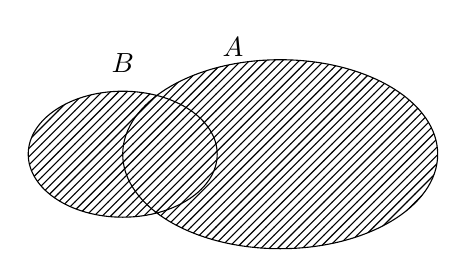
\begin{tikzpicture}[scale=0.8]
	\def\firstven{(0,0) ellipse (1.5cm and 1cm)}
	\def\secondven{(2.5,0) ellipse (2.5cm and 1.5cm)}
	\begin{scope}
		\fill[pattern=north east lines] \firstven \secondven;
	\end{scope}
	\draw \firstven \secondven;%\thirdven;
	\draw
	(0,1.75)node[below]{$B$}
	(1.75,2)node[below]{$A$}
	%	(0.75,0)node[below]{$A\cap B$}
	;
\end{tikzpicture}
}
	\loigiai{
Theo lý thuyết, phần gạch chéo là biểu diễn của tập hợp $A \cup B$.		
	}
\end{ex}

\begin{ex}%[0T6B3-3]%[Dự án đề kiểm tra HKI1 NH22-23- Nguyễn Ngọc Nguyên]%[THPT Tân Bình]
	Thống kê số bàn thắng trong các trận đấu tại WORLD CUP $2022$ tính đến ngày $30/11/2022$ được ghi lại trong bảng tần số sau
	\begin{center}
		\begin{tabular}{|p{4cm}|c|c|c|c|c|c|c|c|c|}
			\hline 
			\centering
			số bàn thắng	&$0$	&$1$	&$2$	&$3$ &$4$ &$5$ & $6$& $7$ & $8$ \\
			\hline 
			\centering
			số trận	&$5$	&$6$	&$12$	&$5$ &$1$ &$4$ &$1$& $1$ & $1$ \\
			\hline 
		\end{tabular}
	\end{center}
Mốt của bảng số liệu trên là
	\choice
	{\True $2$}
	{$12$}
	{$1$}
	{$8$}
	\loigiai{
		Từ bảng ta có số liệu $2$ có tần số lớn nhất là $12$, do đó mốt của mẫu số liệu này là $2$.
	}
\end{ex}

\Closesolutionfile{ans}
%\begin{center}
%	\textbf{ĐÁP ÁN}
%	\inputansbox{10}{ans/ans}	
%\end{center}




\begin{center}
	\textbf{PHẦN 2 - TỰ LUẬN}
\end{center}








\begin{bt}%[0T3B1-1]%[Dự Án Đề Thi HK1-K10-2022-2023-THPT Tân Bình]%[TheHung Nguyen]
	Tìm tập xác định của hàm số sau $y=\sqrt{-3x+2}$.
	\loigiai{Điều kiện xác định $-3x+2\ge 0\Leftrightarrow x\le \dfrac{2}{3}$.\\
		Vậy tập xác định $\mathscr{D}=\left[\dfrac{2}{3};+\right)$
	}
\end{bt}

\begin{bt}%[0T3B2-3]%[Dự Án Đề Thi HK1-K10-2022-2023-THPT Tân Bình]%[TheHung Nguyen]
		Vẽ đồ thị hàm số $y=x^2-6 x+5$.
	\loigiai{\begin{enumerate}[$ \star $]
			\item Tập xác định $\mathscr{D}=\mathbb{R}$.
			\item Trục đối xứng $x=-\dfrac{b}{2a}=3$. 
			\item Tọa độ đỉnh $S(3;-4)$.
			\item Giao với trục $Ox$ tại điểm $(1;0)$ và $(5;0)$.
			\item Bảng giá trị
			\begin{center}
				\begin{tabular}{|c|l|l|l|l|}
					\hline
					$x$& $1$ & $2$ & $3$ & $5$ \\ 
					\hline
					$y=x^2-6x+5$& $0$ & $-3$ & $-4$ & $0$ \\ 
					\hline
				\end{tabular}
			\end{center}
			\item Đồ thị
			\begin{center}
				\begin{tikzpicture}[scale=1, font=\footnotesize, line join=round, line cap=round, >=stealth]
					\def\xmin{-1}\def\xmax{6}\def\ymin{-5}\def\ymax{1}
					\draw[->] (\xmin-0.2,0)--(\xmax+0.2,0) node[below] {\footnotesize $x$};
					\draw[->] (0,\ymin-0.2)--(0,\ymax+0.2) node[right] {\footnotesize $y$};
					\draw (0,0) node [below left] {\footnotesize $O$};
					\foreach \x in {-1,1,4,5,6}\draw (\x,0.1)--(\x,-0.1) node [below] {\footnotesize $\x$};
					\foreach \x in {3}\draw (\x,0.1)--(\x,-0.1) node [below left] {\footnotesize $\x$};
					\foreach \x in {2,3}\draw (\x,0.1)--(\x,-0.1) node [below left] {\footnotesize $\x$};
					\foreach \y in {-5,-4,-3,-2,-1,1}\draw (0.1,\y)--(-0.1,\y) node [left] {\footnotesize $\y$};
					\clip (\xmin,\ymin) rectangle (\xmax,\ymax);
					\draw[smooth,samples=200,domain=\xmin:\xmax] plot (\x,{1*((\x)^2)+-6*\x+5});
					\draw[dashed] (3.0,0)--(3.0,-4.0)--(0,-4.0);\fill (3.0,-4.0) circle (1pt);
					\draw[dashed] (2,0)--(2,-3.0)--(0,-3.0);\fill (2.0,-3.0) circle (1pt);
				\end{tikzpicture}
			\end{center}
		\end{enumerate}		
	}
\end{bt}

\begin{bt}%[0T5B1-4]%[Dự Án Đề Thi HK1-K10-2022-2023-THPT Tân Bình]%[TheHung Nguyen]
		Cho hình chữ nhật $ABCD$ có $AB=5a$, $BC=12 a$. Xác định và tính độ dài véc-tơ $|\overrightarrow{AB}+\overrightarrow{AD}|$ theo $a$.
	\loigiai{
		\immini{Xét $\triangle ABC$ vuông tại $B$, ta có\\		
			 $AC^2=AB^2+AC^2=25a^2+144a^2=169a^2\Rightarrow AC=13a$.\\
			Ta có $|\overrightarrow{AB}+\overrightarrow{AD}|=|\overrightarrow{AC}|=13a$.
		}{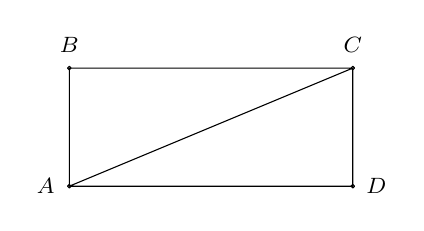
\begin{tikzpicture}[scale=.75, font=\footnotesize, line join=round, line cap=round, >=stealth]
				\def\a{2}
				\def\b{4.8}
				\draw (0,0) coordinate (A)--++(0:\b) coordinate (D)--++(90:\a) coordinate (C)--++(180:\b)coordinate (B)--(0,0)  (A)--(C);
				\foreach \x/\y in {A/180,B/90,C/90,D/0}
				{\draw (\x) circle (0.03cm) + (\y:0.4cm) node {$\x$};
				}
		\end{tikzpicture}}
		
	}
\end{bt}

\begin{bt}%[0T5B3-2]%[Dự Án Đề Thi HK1-K10-2022-2023-THPT Tân Bình]%[TheHung Nguyen]
		Cho tam giác $ABC$. Gọi $I$ là điểm trên cạnh $BC$ sao cho $IC=2IB$. Chứng minh rằng $3\overrightarrow{AI}=2\overrightarrow{AB}+\overrightarrow{AC}$.
	\loigiai{
	\immini{Ta có $I$ thuộc cạnh $BC$ và $IC=2IB\Rightarrow 2\overrightarrow{IB}+\overrightarrow{IC}=\overrightarrow{0}$.
		Ta có 
		\begin{eqnarray*}
			2\overrightarrow{AB}+\overrightarrow{AC} &=& 2\overrightarrow{AI}+2\overrightarrow{IB}+\overrightarrow{AI} +\overrightarrow{IC} \\
			&=& 3\overrightarrow{AI}+ 2\overrightarrow{IB}+\overrightarrow{IC}\\
			&=&  3\overrightarrow{AI}.
		\end{eqnarray*}
	}{\begin{tikzpicture}[scale=.75, font=\footnotesize, line join=round, line cap=round, >=stealth]
			\def\a{5}
			\def\b{4}
			\draw (0,0) coordinate (B)--++(0:\b) coordinate (C)--++(120:\a) coordinate (A)--(0,0);
			\path ($(B)!1/3!(C)$)coordinate (I);
			\foreach \x/\y in {A/90,B/180,C/0,I/-90}
			{\draw (\x) circle (0.03cm) + (\y:0.4cm) node {$\x$};
			}
	\end{tikzpicture}}
	
}
\end{bt}



\begin{bt}%[0T3B2-6]%[Dự Án Đề Thi HK1-K10-2022-2023-THPT Tân Bình]%[TheHung Nguyen]
		Trong môn cầu lông, khi phát cầu, người chơi cần đánh cầu qua khỏi lưới sang phía sân đối phương và không được để cho cầu rơi ngoài biên (xem hình 10).\\
	Trong mặt phẳng toạ độ $Oxy$, chọn điểm có toạ độ $\left(0; y_0\right)$ là điểm xuất phát thì phương trình quỹ đạo của cầu lông khi rời khỏi mặt vợt là $$y=\dfrac{-g \cdot x^2}{2 \cdot v_0^2 \cdot \cos ^2 \alpha}+\tan (\alpha) x+y_0.$$ trong đó:\\
	\begin{itemize}
		\item $g$ là gia tốc trọng trường; $a$ là góc phát cầu (so với phương ngang của mặt đất);
		\item $v_0$ là vận tốc ban đầu của cầu; $y_0$ là khoảng cách từ vị trí phát cầu đến mặt đất.
	\end{itemize}

\begin{center}
	
	%==========================================
	\begin{tikzpicture}[line join=round, line cap=round,scale=1,transform shape]
		%======màu cầu lông
\definecolor{beige}{rgb}{0.96, 0.96, 0.86}
\definecolor{deepskyblue}{rgb}{0.0, 0.75, 1.0}
\definecolor{battleshipgrey}{rgb}{0.52, 0.52, 0.51}
%============màu vẽ vợt
\definecolor{ecru}{rgb}{0.76, 0.7, 0.5}
\definecolor{ballblue}{rgb}{0.13, 0.67, 0.8}
\definecolor{bittersweet}{rgb}{1.0, 0.44, 0.37}
\usetikzlibrary{patterns}
	\usetikzlibrary{calc,angles,quotes,arrows,angles,decorations.markings}
	\tikzset{
	ex_markstyle/.style={},
	ex_mark/.style  n args={1}{decoration={ markings, %
			mark= at position 0.5 with
			with{
				\ifnum#1=1
				\draw[ex_markstyle] (0pt,-2pt) -- (0pt,2pt);
				\fi
				\ifnum#1=2
				\draw[ex_markstyle] (-1pt,-2pt) -- (-1pt,2pt);
				\draw[ex_markstyle] (1pt,-2pt) -- (1pt,2pt);
				\fi
				\ifnum#1=3
				\draw[ex_markstyle] (-2pt,-2pt) -- (-2pt,2pt);
				\draw[ex_markstyle] (0pt,-2pt) -- (0pt,2pt);
				\draw[ex_markstyle] (2pt,-2pt) -- (2pt,2pt);
				\fi
				\ifnum#1=4
				\draw[ex_markstyle] (-1pt,-1pt) -- (1pt,1pt);
				\draw[ex_markstyle] (-1pt,1pt) -- (1pt,-1pt);
				\fi
		} },
		pic actions/.append code=\tikzset{postaction=decorate}},
}


		\clip (-6,-2) rectangle (6,3.5);
		
		\tikzset{cau_long/.pic={
				\def\c{
					(-1.32,-.45)
					..controls +(-145:1.4) and +(-125:1.4) ..(-.6,-1.2)
					--cycle
					;}
				\draw[fill=battleshipgrey] \c;
				\draw%[color=battleshipgrey,line width=.5]
				(-1.22,-.35)--(-.5,-1.1)--(1.5,-.2)--(1.8,.22)--(1.2,.16)%1
				--(1.4,.7)--(.8,.6)%2
				--(.9,1.1)--(.4,1)%3
				--(.5,1.5)--(0.05,1.3)%4
				--(.1,1.9)--(-.35,1.65)--cycle
				;
				\draw (1.2,.16)--(-.65,-.92) (.8,.6)--(-.78,-.8) (.4,1)--(-.95,-.62) (0.05,1.3)--(-1.1,-.48) (-.95,.22)--(.1,-.8);
				
		}}
		
		%================VẼ VỢT
		\tikzset{cai_vot/.pic={
				\def\D{
					(.03,-1.4)--(.35,-1.4)--(.34,-2.85)
					..controls +(-75:.3) and +(-115:.3) ..(.03,-2.85)--cycle;}
				\fill[black] \D;
				\draw \D;
				
				\def\C{ 
					(-.45,0)..controls +(-65:.1) and +(95:1) ..(.05,-1.4)--(.15,-1.4)
					..controls +(85:.2) and +(-50:.6) ..(-.35,0)--cycle
					(.7,0)..controls +(-65:.1) and +(95:.7) ..(.22,-1.4)--(.33,-1.4)
					..controls +(95:.6) and +(-130:.3) ..(.85,0)--cycle
					;
				}
				\fill[bittersweet] \C;
				\draw \C;
				%-----------------sọc chéo
				\def\S{
					(.03,-1.5)..controls +(-35:.1) and +(145:.1) ..(.35,-1.6)
					(.03,-1.7)..controls +(-35:.1) and +(145:.1) ..(.35,-1.8)
					(.03,-1.8)..controls +(-35:.1) and +(145:.1) ..(.35,-1.9)
					(.03,-2)..controls +(-35:.1) and +(145:.1) ..(.35,-2.1)
					(.03,-2.1)..controls +(-35:.1) and +(145:.1) ..(.35,-2.2)
					(.03,-2.3)..controls +(-35:.1) and +(145:.1) ..(.35,-2.4)
					(.03,-2.4)..controls +(-35:.1) and +(145:.1) ..(.35,-2.5)
					(.03,-2.6)..controls +(-35:.1) and +(145:.1) ..(.35,-2.7)
					(.03,-2.7)..controls +(-35:.1) and +(145:.1) ..(.35,-2.8)
					(.03,-2.85)..controls +(-35:.1) and +(145:.1) ..(.35,-2.95)
					;}
				\draw[bittersweet] \S;
				
				\def\N{ 
					(2.72,-.195)  arc (0:360:1.48 cm and 1.2cm)
					;
				}
				\def\T{ 
					(2.65,-.2)  arc (0:360:1.4 cm and 1.1cm)
					;
				}
				\fill[rotate=90,ballblue] \N;
				\draw[rotate=90] \N;
				\fill[rotate=90,white] \T;
				
				\draw[rotate=90,ecru!70!black,draw=gray!50, thick,pattern color=gray!50,
%				preaction={pattern=flexible grid},
				minimum width=30mm, minimum height=20mm,
				below right]\T;
				\draw[rotate=90] \T;
		}}
		%============================================
		
		\def\xmin{-3.5} \def\xmax{5.7}
		\def\ymin{-1.5} \def\ymax{2} 
		\draw[->] (\xmin,-1)--(\xmax,-1) node [above left]{\tiny $x$};
		\draw[->] (-3,\ymin)--(-3,\ymax) node [left]{\tiny $y$};
		\node at (-3,-1) [below left]{\tiny $O$};
		\draw[dashed] 
		(-3,0)
		..controls +(50:2.3) and +(150:1) .. (4.5,-1)
		(-3,0)
		..controls +(50:2.3) and +(150:1) .. (2.5,-1)
		(-3,0)
		..controls +(60:1.2) and +(140:.8) .. (1.2,-1)
		;%đường đi cầu lông
		
		\draw
		(-3,0)
		..controls +(50:2.3) and +(150:1) .. (2,-1);%đường đi cầu lông
		\draw[<->](-3,-1.1)--(-.3,-1.1);
		\node at (-.3,-.5) [left]{\tiny $1{,}524$ m};
		\node at (-1.7,-1.1) [below]{\tiny $4$ m};
		\node at (-.5,-1.1) [below]{\tiny lưới phân cách};
		\draw[line width=.7] (-.3,-1)circle (.5pt)--(-.3,0)circle (.5pt);
		
		\draw[fill=black] (4.5,-1) circle (.5pt);
		\node at (4.5,-1) [below]{\tiny điểm biên ngoài};
		\draw[fill=black] (1.2,-1) circle (.5pt);
		\node at (1.2,-1) [below]{\tiny điểm biên trong};
		\node at (1.8,0) [below]{\tiny hợp lệ};
		\node at (.25,0) [below]{\tiny hỏng};
		\node at (3.4,0) [below]{\tiny hỏng};
		
		\path
		(-3,-.5)pic[scale=.2,rotate=50]{cai_vot}
		(-2.95,0)pic[scale=.1]{cau_long}
		;
		
		
	\end{tikzpicture}	
\end{center}
	 Một người đang tập chơi cầu lông, có khuynh hướng phát cầu với góc $30^{\circ}$ (so với mặt đất) biết cầu rời mặt vợt ở độ cao $0{,}8$m so với mặt đất và vận tốc xuất phát của quả cầu là $8$m/s (bỏ qua sức cản của gió xem quỹ đạo của cầu luôn nằm trong mặt phẳng phẳng đứng, lấy $g$ là $9{,}8$m/s$^2$). Người ấy phát cầu như thế có bị xem là hỏng không? Vì sao? (biết điểm biên trong và điểm biên ngoài lần lượt cách $O$ là $5{,}98 $m  và $9{,}94$m).
	 \begin{center}
	 	\definecolor{beige}{rgb}{0.96, 0.96, 0.86}
	 	\definecolor{deepskyblue}{rgb}{0.0, 0.75, 1.0}
	 	\definecolor{battleshipgrey}{rgb}{0.52, 0.52, 0.51}
	 	\begin{tikzpicture}[line join=round, line cap=round,scale=1,transform shape]
	 		\clip (-6,-2) rectangle (4,3.5);
	 		
	 		\tikzset{cau_long/.pic={
	 				\def\c{
	 					(-1.32,-.45)
	 					..controls +(-145:1.4) and +(-125:1.4) ..(-.6,-1.2)
	 					--cycle
	 					;}
	 				\draw[fill=battleshipgrey] \c;
	 				\draw%[color=battleshipgrey,line width=.5]
	 				(-1.22,-.35)--(-.5,-1.1)--(1.5,-.2)--(1.8,.22)--(1.2,.16)%1
	 				--(1.4,.7)--(.8,.6)%2
	 				--(.9,1.1)--(.4,1)%3
	 				--(.5,1.5)--(0.05,1.3)%4
	 				--(.1,1.9)--(-.35,1.65)--cycle
	 				;
	 				\draw (1.2,.16)--(-.65,-.92) (.8,.6)--(-.78,-.8) (.4,1)--(-.95,-.62) (0.05,1.3)--(-1.1,-.48) (-.95,.22)--(.1,-.8);
	 				
	 		}}
	 		
	 		\draw (-3,0)
	 		..controls +(50:2.3) and +(150:1) .. (3,-1);%đường đi cầu lông
	 		\draw[->](-3,0)--(-2.5,.35);
	 		\draw[dashed](-3,0)--(-1.5,0);
	 		\node at (-2,0) [above]{\tiny $\alpha =30^\circ$};
	 		\draw[fill=black] (3,-1) circle (.5pt);
	 		\node at (3,-1) [below]{\tiny điểm chạm đất};
	 		\node at (-3,0) [left]{\tiny $y_\circ=0{,}8$ m};
	 		\node at (-.5,-1) [above]{\tiny $y=\dfrac{-g\cdot x^2}{2v_\circ^2\cdot \cos^2\alpha}+\tan (\alpha) \cdot x+y_\circ$};
	 		\path
	 		(-1.5,.7)pic[scale=.1,rotate=-30]{cau_long};
	 		
	 		\def\xmin{-3.5} \def\xmax{4}
	 		\def\ymin{-1.5} \def\ymax{2} 
	 		\draw[->] (\xmin,-1)--(\xmax,-1) node [above left]{\tiny $x$};
	 		\draw[->] (-3,\ymin)--(-3,\ymax) node [left]{\tiny $y$};
	 		\node at (-3,-1) [below left]{\tiny $O$};	 		
	 	\end{tikzpicture}
	 \end{center}
	 \loigiai{
	 Ta có 	  $\alpha =30^{\circ}$, $v_0=8$m/s, $g=9{,}8$m/s$^2$), khi đó phương trình quỹ đạo của cầu là
 $$y=-\dfrac{9{,}8x^2}{2\cdot 8^2\cdot\cos^2\left(30^{\circ}\right)}+\tan\left(30^{\circ}\right)\cdot x+0{,}8=\dfrac{-4{,}9}{48}x^2+\dfrac{\sqrt 3}3x+0{,}8.$$ 
 Vị trí cầu rơi chạm đất là giao điểm của parabol và trục hoành nên giải phương trình $\dfrac{-4,9}{48} x^2+\dfrac{\sqrt{3}}{3} x+0,8=0$ ta được $x_1 \approx-1,15$ và $x_2 \approx 6,81$.\\
 Do vị trị rơi cách $O$ một khoảng  $6,81$m nên giao bóng hợp lệ. 
 }
\end{bt}


\begin{bt}%[0T5K4-4] %[Dự Án Đề Thi HK1-K10-2022-2023-THPT Tân Bình]%[TheHung Nguyen]
	Cho tam giác $ABC$ vuông tại $A$ có $AB=a$, $AC=a\sqrt{2}$. Gọi $M$ và $N$ là các điểm thỏa: $\overrightarrow{MB}+\overrightarrow{MC}=\overrightarrow{O}; \overrightarrow{AN}=2 \overrightarrow{BN}$. Chứng minh $A M \perp  CN$.
	\loigiai{
	\immini{Ta có $\overrightarrow{MB}+\overrightarrow{MC}=\overrightarrow{O}\Rightarrow M$ là trung điểm của $BC$.\\
		Khi đó $\overrightarrow{AM}=\dfrac{1}{2}\overrightarrow{AB}+\dfrac{1}{2}\overrightarrow{AC}$.
		Ta có \begin{eqnarray*}
			&& \overrightarrow{AN}=2 \overrightarrow{BN} \\
			&\Leftrightarrow& \overrightarrow{AC}+\overrightarrow{CN}=2\overrightarrow{BC}+2\overrightarrow{CN} \\
			&\Leftrightarrow& \overrightarrow{AC}=2\overrightarrow{BA}+2\overrightarrow{AC}+\overrightarrow{CN}\\
			&\Leftrightarrow& \overrightarrow{CN}=2\overrightarrow{AB}-\overrightarrow{AC}.
		\end{eqnarray*}
	Ta có \begin{eqnarray*}
		\overrightarrow{AM}\cdot \overrightarrow{CN}&=&\dfrac{1}{2}\left(\overrightarrow{AB}+\overrightarrow{AC}\right)\left(2\overrightarrow{AB}-\overrightarrow{AC}\right)   \\
		&=& \dfrac{1}{2}\left(2AB^2-\overrightarrow{AB}\cdot\overrightarrow{AC}+2\overrightarrow{AB}\cdot\overrightarrow{AC}-AC^2\right) \\
		&=& 2a^2-2a^2=0.
	\end{eqnarray*}
Do đó $A M \perp  CN$.
	}{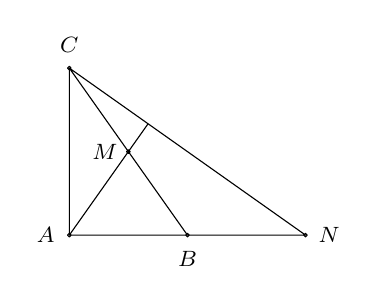
\begin{tikzpicture}[scale=.75, font=\footnotesize, line join=round, line cap=round, >=stealth]
			\def\a{2}
			\pgfmathsetmacro{\b}{\a*sqrt(2)}
			\path (0,0)coordinate (A)--++(90:\b)coordinate (C)
			 (0,0)--++(0:\a)coordinate (B)--++(0:\a) coordinate (N)
			
		($(B)!.5!(C)$)coordinate (M)  ($(N)!(A)!(C)$)coordinate (K)
		;	
			
		\draw (C)--(A)--(N)--(C)--(B) (A)--(M)--(K);
			\foreach \x/\y in {A/180,B/-90,C/90,N/0,M/180}
			{\draw (\x) circle (0.03cm) + (\y:0.4cm) node {$\x$};
			}
	\end{tikzpicture}}
	
}
\end{bt}


